\section{GAN}

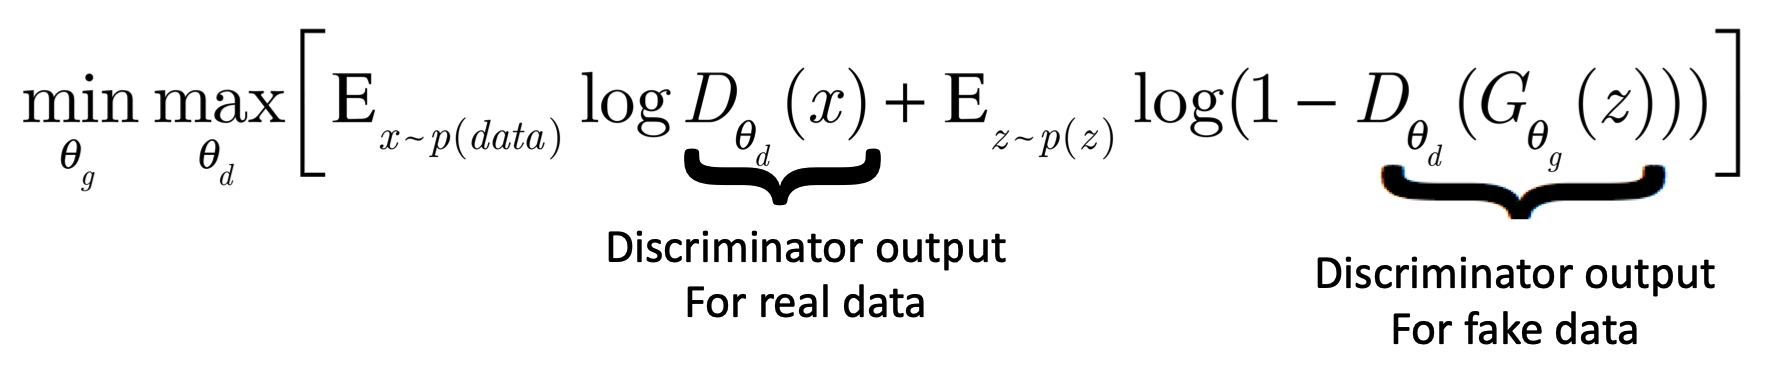
\includegraphics[width=0.9\columnwidth]{images/gan}

This has bad training properties so we use this instead

$$
\max \log D(G(z))
$$

\begin{itemize}
  \item The Discriminator wants to maximize this objective so that D(x) is close to 1 (real) and D(G(z)) is close to 0 (fake)
\item The Generator wants to minimize this objective such that D(G(z)) is close to 1 (discriminator is fooled into thinking generated G(z) is real)
\end{itemize}


\textbf{CycleGan}

Translates from one domain to another without pairing data.
Uses "cycle consistency loss": if X translates to Y, then Y should translate to X

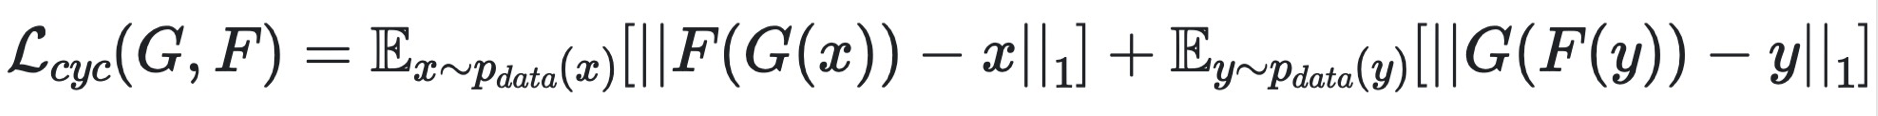
\includegraphics[width=0.9\columnwidth]{images/cyclegan_loss}
